\needspace{3cm}
\subsection{Aclaración del Problema}
Desde el punto de vista de diseño mecánico del producto, el objetivo es diseñar un sistema embebido que debe ocupar las mínimas dimensiones. Estas dimensiones están limitadas por tres factores:

\begin{itemize}
    \item El tamaño y forma de los dispositivos electrónicos contenidos.
    \item El espacio que ocupan los sistemas auxiliare, en este caso baterías y refrigeración.
    \item El espacio que ocupan los actuadores a fin de garantizar dos grados de libertad.
\end{itemize}

Se conocen las especificaciones técnicas del mínimo de sensores a utilizar y el tamaño del microcontrolador seleccionado por el equipo de diseño electrónico, el resto de elementos quedan a criterio del equipo de diseño mecánico.

Más aun, se debe diseñar el sistema para manufactura en masa en impresoras FDM (\textit{Filament Deposition Modeling}).

\subsubsection{Especificaciones de Componentes Electrónicos}
\begin{itemize}
    \needspace{3cm}
    \item \textbf{ESP32 CAM12}
    \begin{itemize}
        \item Dimensiones: 40.5mm x 27mm x 4.5mm
        \item Voltaje de alimentación: 5V
        \item Consumo de energía: Menos de 800mW en funcionamiento, tan bajo como 6mA en modo de suspensión profunda
        \item Temperatura de funcionamiento: -20 ℃ ~ 85 ℃
    \end{itemize}
    
    \needspace{3cm}
    \item \textbf{HC-SR501345}
    \begin{itemize}
        \item Dimensiones: 32mm x 24mm
        \item Voltaje de alimentación: 4.5V - 20V (5V recomendado)
        \item Consumo de energía: 65mA
        \item Temperatura de funcionamiento: -20 °C ~ +70 °C
    \end{itemize}

    \needspace{5cm}
    \item \textbf{MQ-135678}
    \begin{itemize}
        \item Dimensiones: 18mm de diámetro, 17mm de alto sin contar los pines
        \item Voltaje de alimentación: 2.5V ~ 5.0V
        \item Consumo de energía: No especificado
        \item Temperatura de funcionamiento: No especificado
    \end{itemize}
\end{itemize}

\subsubsection{Descomposición del Problema}
Tomando en cuenta las limitaciones del producto se puede descomponer el sistema en cuatro subsistemas principales: Procesamiento de las señales de los sensores, administración de energía, sistema de movimiento y gestión termica o direccionamiento de aire. La Figura \ref{fig:analisis_funcional} describe por medio de un diagrama de bloques la interacción entre estos subsistemas: La energía eléctrica entra al bloque de administración de energía, dentro del mismo la energía se puede almacenar en baterías, alternar su naturaleza o nivel. Este bloque se conecta a todos los subsistemas: Procesamiento, movimiento y direccionamiento de aire. A su vez, el bloque de procesamiento puede o no controlar los sistemas de direccionamiento de aire y de movimiento.

\begin{figure}[H]
\centering
\begin{adjustbox}{width=\linewidth}
  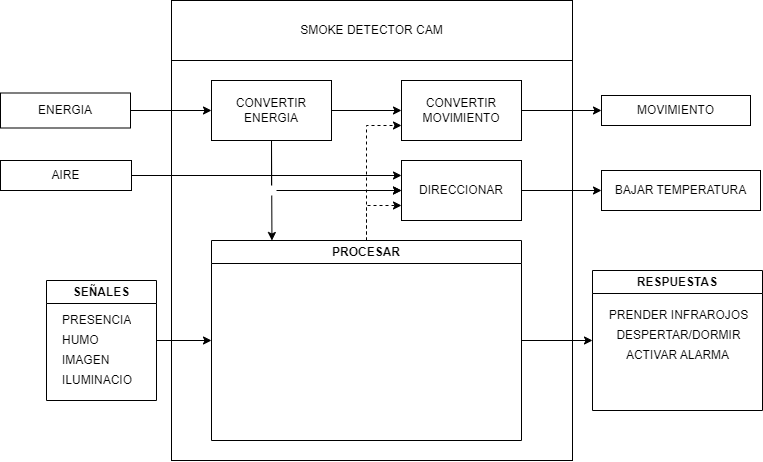
\includegraphics{media/analisis_sistema.png}
\end{adjustbox}
\caption{\label{fig:analisis_funcional}Análisis Funcional del Sistema.}
\end{figure}

\subsubsection{Subproblemas Críticos}
\begin{enumerate}[label=\alph*)]
    \item Administración de Energía
        \needspace{3cm}
        \begin{enumerate}[label=\Roman*)]
            \item \textbf{Selección de cables y conectores adecuados:} Elegir cables y conectores de alta calidad y con capacidades de corriente adecuadas para minimizar la pérdida de energía y garantizar una transmisión de energía eficiente.
    
            \needspace{3cm}
            \item \textbf{Enrutamiento de cables:} Planificar cuidadosamente la disposición de los cables dentro del dispositivo para evitar cruces, pliegues o torsiones excesivas que puedan causar pérdida de energía o dañar los cables con el tiempo.
    
            \needspace{3cm}
            \item \textbf{Protección contra cortocircuitos:} Implementar mecanismos de protección, como fusibles o disyuntores, para prevenir cortocircuitos que podrían dañar los cables y afectar la administración de energía.
    
            \needspace{3cm}
            \item \textbf{Acceso y mantenimiento:} Diseñar el sistema mecánico de manera que sea fácil acceder a los cables y conectores para el mantenimiento y la sustitución, si es necesario, sin tener que desmontar todo el dispositivo.
    
            \item \textbf{Selección de batería:} La elección de la batería se realiza cuidadosamente, considerando los requisitos de energía específicos de los actuadores del dispositivo, como motores, sensores y otros componentes, y asegurando que la batería seleccionada tenga la capacidad adecuada para suministrar la energía requerida de manera constante y confiable. Además, se evalúa minuciosamente el tamaño y la forma de la batería para garantizar su integración eficiente en el diseño mecánico del dispositivo, optimizando así el espacio disponible y manteniendo un equilibrio adecuado entre la capacidad de la batería y las limitaciones de tamaño del dispositivo.
        \end{enumerate}
        
    \item Sistema de Movimiento
    \begin{enumerate}[label=\Roman*)]
        \item \textbf{Requisitos de movimiento:} Define claramente los requisitos de movimiento del dispositivo, incluyendo los rangos de movimiento, las velocidades y las aceleraciones necesarias para cumplir con su función prevista.
        
        \item \textbf{Selección de actuadores:} Elije los actuadores adecuados para controlar el movimiento en los dos grados de libertad. Considera motores eléctricos, motores paso a paso, actuadores lineales o cualquier otro tipo de actuador que se adapte a tus necesidades.
        
        \item \textbf{Mecanismos de control de movimiento:} Analizar la incorporación de sistemas de guía o mecanismos para garantizar un movimiento suave y preciso en el rango requerido. 
        
        \item \textbf{Costos:} Gestiona el presupuesto disponible para el proyecto y selecciona componentes y materiales que se ajusten a él sin comprometer la calidad y el rendimiento del dispositivo.
        
        \item \textbf{Montaje:} Planificar el montaje de los actuadores tomando en cuenta el proceso de fabricación y herramientas de montaje.
    \end{enumerate}

\item Gestión Térmica
    \begin{enumerate}[label=\Roman*)]
        \needspace{3cm}
        \item \textbf{Selección de ventiladores o actuadores:} Seleccionar los ventiladores o actuadores adecuados basándose en los requisitos de flujo de aire del dispositivo y las características de capacidad, eficiencia y durabilidad.

        \needspace{3cm}
        \item \textbf{Distribución del flujo de aire:} Diseñar y asegurarse de que los conductos de aire estén configurados de manera que el flujo de aire se distribuya de manera uniforme en todo el dispositivo.

        \needspace{3cm}
        \item \textbf{Espacio y restricciones de tamaño:} Diseñar el sistema de direccionamiento de aire teniendo en cuenta las limitaciones de espacio y tamaño para asegurarse de que se ajuste correctamente en el dispositivo embebido.

        \needspace{3cm}
        \item \textbf{Gestión de costos:} Gestionar el presupuesto del proyecto y seleccionar componentes y materiales que se ajusten a él sin comprometer la calidad y el rendimiento del sistema de gestión térmica.

        \needspace{3cm}
        \item \textbf{Planificación de fabricación y montaje:} Planificar cómo se fabricarán los componentes del sistema de dirección de aire y cómo se ensamblarán de manera eficiente, eligiendo procesos de fabricación adecuados y herramientas de montaje.
    \end{enumerate}
\end{enumerate}

\needspace{3cm}
\subsection{Búsqueda Externa}
\subsubsection{Análisis de Literatura}
Se dividió el análisis de literatura en base a los tres problemas principales que se desea solucionar:

    \begin{enumerate}[label=\alph*)]
    \item \textbf{Administración de Energía} \\
    Esta sección desarrolla dos aspectos fundamentales del diseño de productos electrónicos: La gestión de cables y la selección de baterías.  La gestión de cables cumple dos funciones esenciales: Garantizar la seguridad de los cables en una aplicación y dirigirlos a través de puntos de acceso. 

    \begin{enumerate}[label=\Roman*)]
    \item \textbf{Selección de Baterias} \\
    \begin{itemize}
    
    \needspace{8cm}
    \item \textbf{Baterías No Recargables}
    
        \begin{table}[H]
        \centering
        \begin{tabularx}{\textwidth}{|c|X|X|X|}
        \hline
        \textbf{Tipo} & \textbf{Ventajas} & \textbf{Desventajas} & \textbf{Usos} \\
        \hline
        Baterías Alcalinas & Tamaño pequeño, Eficientes, Baja fuga & Costo elevado & Linternas, mandos a distancia, pequeños electrodomésticos \\
        \hline
        Baterías de Botón & Livianas, alta densidad, bajo costo, alto voltaje nominal & Requiere un soporte, baja capacidad de corriente & Relojes, relojes de pared, productos electrónicos en miniatura \\
        \hline
        \end{tabularx}
        \caption{Análisis de Baterías No Recargables}
        \label{tab:baterias_no_recargables}
        \end{table}

    \needspace{4cm}
    \item \textbf{Baterías Secundarias Comunes}
    
        \begin{table}[H]
        \centering
        \begin{tabularx}{\textwidth}{|c|X|X|X|X|}
        \hline
        \textbf{Tipo} & \textbf{Plomo-Ácido} & \textbf{NiCd} & \textbf{NiMH} & \textbf{Li-Ion*} \\
        \hline
        Voltaje de Celda & 2V & 1.2V & 1.2V & 3.2-3.6V \\
        \hline
        Voltaje de Corte de Descarga & 1.75V & 1.00V & 1.00V & 2.50V \\
        \hline
        Corriente de Descarga & 5C & 20C & 5C & 2C o >30C \\
        \hline
        Vida Útil de Ciclo & 200-300 & 1000 & 300-500 & 500-1000 \\
        \hline
        Auto-Descarga / mes & 5\% & 20\% & 30\% & <5\% \\
        \hline
        Temperatura de Carga & -20 a 50°C & 0 a 45°C & 0 a 45°C & 0 a 45°C \\
        \hline
        Temperatura de Descarga & -20 a 50°C & -20 a 65°C & -20 a 65°C & -20 a 60°C \\
        \hline
        Requisito de Mantenimiento & 3-6 meses & Descarga completa cada 90 días en uso completo & Descarga completa cada 90 días en uso completo & No requerido \\
        \hline
        Costo & Bajo & Moderado & Moderado & Alto \\
        \hline
        \end{tabularx}
        \caption{Análisis de Baterías Recargables}
        \label{tab:baterias_recargables}
        \end{table}
        
        La Tabla \ref{tab:baterias_recargables} ofrece una comparativa de diferentes tipos de baterías recargables. Las "Plomo-Ácido" son económicas pero requieren mantenimiento regular. Las "NiCd" y "NiMH" son duraderas pero necesitan descargas periódicas. Las "Li-Ion*" son versátiles y sin mantenimiento, pero tienen un costo más elevado; Para uso general las baterías de Li-ion son las más adecuadas debido a la falta de mantenimiento, una larga vida útil de ciclo y una baja auto-descarga. Esto es por qué son populares en muchos aparatos como laptops y teléfonos móviles. Sin embargo, una desventaja es el costo (\cite{tan2020guide}).
        
    \end{itemize}

    \item \textbf{Manejo de Cables} 
    
    Para optimizar el tiempo de operación de su aplicación y evitar costosas reparaciones, es fundamental proteger los cables contra daños directos. Para esta tarea, se puede contar con soluciones como conducciones, envolturas para cables, casquillos de alivio de tensión y cajas de conexiones. Sin embargo, cuando se trata de orientar y administrar múltiples cables de manera eficiente, se consideran otras alternativas, como ser sujeta-cables, clips para cables, envolturas de cable y pasa-cables(\cite{essentraCableManagement}). Estos elementos permiten dirigir estratégicamente los cables.
    Cada una de las soluciones presentadas a continuación es esencial para resolver ciertos problemas cuando se trata de la organización de cables y mejorar la gestión de cables:

    \begin{figure}[H]
    \centering
    \begin{adjustbox}{width=\linewidth/2}
      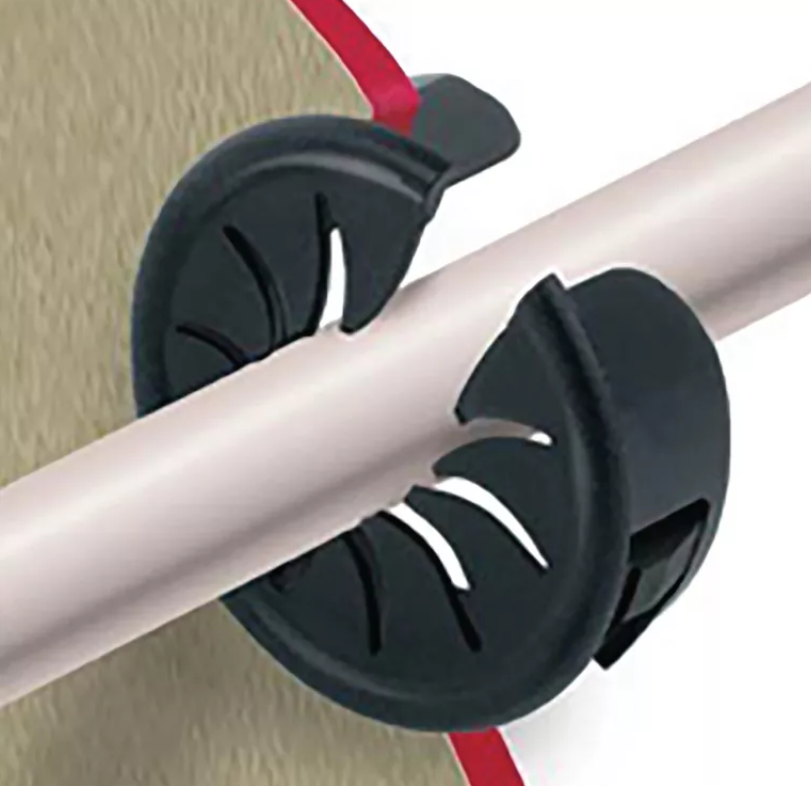
\includegraphics{media/cable_bushings_esentra.png}
    \end{adjustbox}
    \caption{\label{fig:cable_bushings}Arandela para cables.}
    Fuente: \textcite{essentraCableManagement}.
    \end{figure}
    
    \begin{itemize}
    \item \textbf{Arandelas para cables:} Permiten que los cables pasen de manera segura a través de una barrera conductora conectada a tierra, como chapa metálica, un transformador o un interruptor.
    \item \textbf{Clips para cables:} Aseguran los cables en una superficie como se ve en la Figura \ref{fig:cable_bushings}.
    \item \textbf{Abrazaderas para cables:} Proporcionan soporte mientras definen una ruta para los cables a lo largo de una pared o dentro de una aplicación.
    \item \textbf{Correas para cables:} Mantienen un pequeño grupo de cables juntos para mantenerlos organizados.
    \item \textbf{Monturas para correas para cables:} Elemento de fijación para correas para cables, aplicado a superficies.
    \item \textbf{Envolturas y fundas para cables:} Organizan los cables en un solo paquete.
    \item \textbf{Glandes para cables:} Evitan daños y fallos en los cables y se utilizan para pasar cables a una carcasa o dispositivo de control. Por lo general, se utilizan en entornos industriales para controlar la curva o evitar que un cable se salga de un sistema.
    \item \textbf{Tubos termorretráctiles:} Aíslan los cables, proporcionando resistencia a la abrasión y protección ambiental. Disponibles en diferentes colores para permitir la codificación por colores.
    \item \textbf{Correas de torsión:} Ideales para circuitos y placas eléctricas. Mantienen los cables en su lugar, alejados de los paneles.
    \end{itemize}
    
    La gestión de cables es crucial para mantener la organización y la seguridad en entornos donde se utilizan cables y alambres. Cada una de estas soluciones desempeña un papel importante en abordar problemas específicos relacionados con la gestión de cables, desde la protección contra daños hasta la organización efectiva. Estos productos y materiales son esenciales para garantizar que los cables funcionen de manera confiable y se mantengan ordenados en diversas aplicaciones, desde entornos industriales hasta aplicaciones domésticas.

    \end{enumerate}

    \item \textbf{Sistema de Movimiento} \\
    Una revisión inicial de literatura permite observar que existen dos soluciones que se pueden dar al problema de movimiento panorámico e inclinación requerido por el sistema: Utilizar directamente dos actuadores en serie que con control de lazo cerrado de posición similar al de \textcite{Yosafat2017} o utilizar algún mecanismo diseñado para este propósito como el que expone \textcite{diff_pan_tilt_youtube}. A estos últimos se los denomina como Generadores de Movimiento Panorámico y de Inclinación, \textit{PTMG} por sus siglas en ingles. La primera solución implicando un incremento de tamaño, precisión y velocidades limitadas mientras que la segunda soluciona todos los problemas de la primera, pero implica una mayor complejidad de diseño (\cite{Alizadeh2010}) y en muchos casos de manufactura.

    Siendo así, inicialmente y en base a la información proporcionada por \textcite{motorSelection} se desarrolló la comparación de motores del Cuadro \ref{tab:motor-comparison}.
    
    \begin{table}[H]
        \centering
        \begin{tabularx}{\textwidth}{|c|c|X|X|X|}
            \hline
            \textbf{Tipo de Motor} & \textbf{Ruido} & \textbf{Mantenimiento} & \textbf{Ventajas} & \textbf{Limitaciones} \\
            \hline
            Motor DC & Alto & Constante & Adecuados para soluciones de bajo costo. Generan ruido eléctrico. Velocidad limitada debido al calentamiento de las escobillas. & Requieren controladores adicionales. \\
            \hline
            Motor Brushless & Bajo & Medio & Eficientes con bajo ruido eléctrico. Alta durabilidad. & Costo inicial más alto. \\
            \hline
            Motor a Paso & Medio & Medio & Posicionamiento preciso, control de velocidad y alto par a bajas velocidades. Alto par de retención. & Requieren un controlador de pasos. \\
            \hline
            Servomotor & Bajo & Poco & Alto par a altas velocidades, variedad en tamaños y opciones rentables. & Rango de movimiento limitado, posibles sacudidas. \\
            \hline
        \end{tabularx}
        \caption{Comparación de Motores}
        \label{tab:motor-comparison}
    \end{table}

    Si se prioriza una operación silenciosa y eficiente, la mejor opción son los motores de corriente continua sin escobillas. Para realizar un posicionamiento preciso y mantener un control de velocidad, los motores paso a paso destacan gracias a su alto conteo de polos. Cuando se requieren capacidades de alta velocidad y alto par, los motores servo se convierten en la elección ideal, especialmente cuando se superan las 2000 rpm. En el caso de opciones económicas, se puede considerar los servos de tamaño pequeño. No obstante, si la búsqueda se enfoca en una solución rentable con niveles de ruido aceptables, los motores de corriente continua tradicionales también pueden ser apropiados. Es importante tener en cuenta que cada tipo de motor presenta sus propias limitaciones, por lo tanto, la elección debe ajustarse a los requisitos y limitaciones específicos del proyecto en cuestión.

    Por otro lado, se identificaron los PTMGs descritos a continuación; Notese que los primeros cuatro hacen uso de sistemas de engranes planetarios. Un sistema de engranajes planetarios está compuesto por un sol, dos planetas, una corona y un portaplanetas. Al activar los engranajes del sol y la corona, se logra el movimiento panorámico directamente a partir de la rotación del portaplanetas. Sin embargo, se necesita un mecanismo intermedio para transferir la rotación del planeta alrededor de su propio eje vertical al eje de inclinación del eje horizontal.
    
    \needspace{4cm}
    \begin{enumerate}[label=\Roman*)]
    \item \textbf{\textit{Bevel-gear train}:} Del mismo modo, los engranajes cónicos pueden transferir la rotación entre dos ejes que se cruzan. En consecuencia, se puede emplear un par de engranajes cónicos de manera simple para llevar a cabo la transmisión de la rotación desde el planeta hasta el eje de inclinación.

    \begin{figure}[H]
    \centering
    \begin{adjustbox}{width=\linewidth/2}
      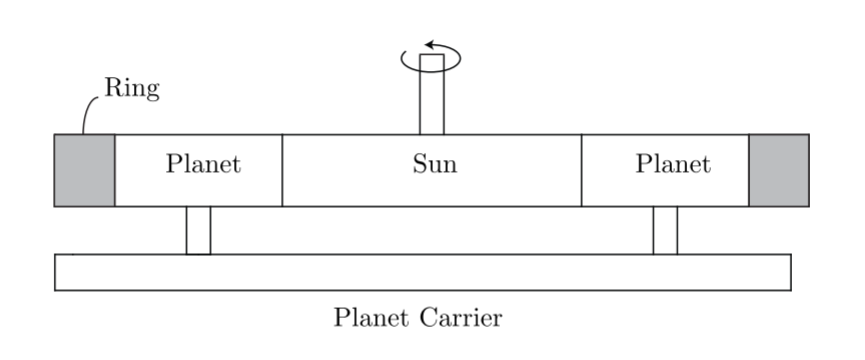
\includegraphics{media/planet_gear.png}
    \end{adjustbox}
    \caption{\label{fig:planet_gear_mechanism}Mecanismo de tren de engranes planetarios.}
    Fuente: \textcite{Yosafat2017}
    \end{figure}
    
    \item \textbf{\textit{Homokinetic joints}:} Se trata de un tipo de conexión cinemática entre dos ejes que se cruzan se conoce como una junta homocinética o junta de velocidad constante (CV). Esto permite la transferencia de velocidad angular, par y potencia con una relación de 1:1. Estos acoplamientos se emplean para convertir el movimiento de rotación del planeta en movimiento de inclinación; Puede tratarse de, por ejemplo, por dos uniones universales o una union Rzeppa.
    
    \item \textbf{\textit{Five-bar linkage}:} Tal como se describe en el nombre, se trata de un mecanismo de cinco barras que produce el movimiento de inclinación por medio del movimiento del planeta.
    
    \item \textbf{\textit{Spherical linkage}:} Este mecanismo se caracteriza por diseñar sus ejes de entrada y salida de manera ortogonal, buscando lograr una relación de velocidad cercana a 1:1.
    
    \item \textbf{\textit{Differential gear train}:} Este PTMG, cuyo diagrama esquemático está la Figura \ref{fig:diff_mechanism}, emplea un tipo distinto de mecanismo de engranaje planetario en comparación con el que se describió inicialmente. El tren de engranajes diferencial es impulsado por dos motores idénticos A y B. El engranaje solar inferior está montado en un eje hueco y es impulsado por el motor A, mientras que el eje del engranaje solar superior, accionado por el motor B, pasa a través del eje hueco; esta disposición permite al diseñador colocar ambos motores en el marco de la base, en la parte inferior. La rotación del marco móvil alrededor del eje vertical produce el movimiento de panorámica, mientras que la rotación de los planetas alrededor de sus ejes proporciona el movimiento de inclinación.

    \begin{figure}[H]
    \centering
    \begin{adjustbox}{width=\linewidth/2}
      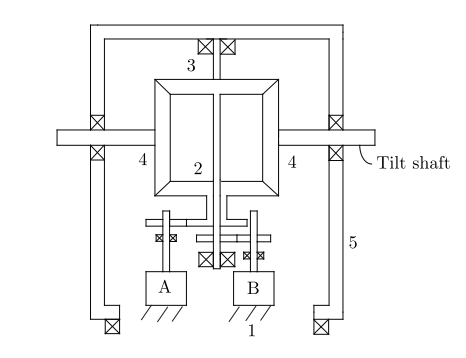
\includegraphics{media/differential_mechanism.png}
    \end{adjustbox}
    \caption{\label{fig:diff_mechanism}Mecanismo de tren de engranes diferencial.}
    Fuente: \textcite{Yosafat2017}
    \end{figure}
    
    \item \textbf{\textit{Hervé's pan-tilt linkage}:} Hervé (2006) citado en \textcite{Yosafat2017} sintetizó varios PTMGs paralelos de dos miembros utilizando la teoría de grupos. Dado que los mecanismos propuestos en (Hervé, 2006) no están excesivamente restringidos, pueden tolerar errores en la fabricación y el ensamblaje. Además, las actuaciones de panorámica e inclinación están desacopladas, es decir, los ejes de panorámica e inclinación pueden ser accionados de manera independiente.
    \end{enumerate}
    
    \item \textbf{Gestión Térmica} \\
    Las tecnologías de gestión térmica se clasifican en sistemas de enfriamiento con contacto directo o indirecto con el fluido de enfriamiento, según si el fluido de enfriamiento entra o no en contacto directo con los componentes que se están enfriando. Dentro de la ventilación directa se considerara solamente la ventilación por aire debido a su bajo costo y popular uso en aparatos de consumo (\cite{zhang2021review}).

    \needspace{3cm}
    \begin{enumerate}[label=\Roman*)]
    \item \textbf{\textit{Directa: Ventilación de Aire de adelante hacia atrás:}} Enfoque de diseño y gestión térmica utilizado en sistemas electrónicos y equipos para disipar el calor generado por los componentes internos de manera eficiente (\cite{Group_2017}). En este enfoque, el flujo de aire fresco entra en el sistema desde el frente (o la parte delantera) del equipo y fluye hacia la parte trasera, pasando a través de los componentes electrónicos y llevando consigo el calor generado. Luego, el aire caliente se expulsa hacia afuera desde la parte trasera del equipo.

    Este método se utiliza para evitar que el aire caliente se mezcle con el aire fresco en el interior del sistema, lo que podría provocar un aumento de la temperatura y, en última instancia, el sobrecalentamiento de los componentes electrónicos. Al mantener un flujo de aire ordenado y unidireccional de frente a atrás, se puede mantener una temperatura adecuada dentro del equipo, lo que es fundamental para garantizar el rendimiento y la fiabilidad de los dispositivos electrónicos, como servidores, sistemas de almacenamiento, enrutadores y conmutadores, entre otros.

        \needspace{3cm}
        \begin{enumerate}[label=\alph*)]
        \item \textbf{Ventiladores en la Parte Trasera:}
        \begin{itemize}
            \item Los ventiladores se colocan directamente detrás del conjunto de placas electrónicas para extraer el calor.
            \item Aunque es eficaz, puede presentar desafíos en cuanto a la filtración del aire.
            \item Adecuado para muchas aplicaciones, pero puede no ser óptimo para procesadores de alta potencia y necesidades de entrada/salida trasera.
        \end{itemize}
    
        \item \textbf{Montaje Horizontal de Placas Electrónicas:}
        \begin{itemize}
            \item Las placas electrónicas se montan horizontalmente con una entrada de aire en la parte frontal izquierda y una salida en la parte trasera izquierda.
            \item Opción que ahorra espacio, especialmente en configuraciones con pocas ranuras.
            \item Menos eficiente en la refrigeración debido a áreas limitadas de entrada y salida (por ejemplo, un chasis de 4U puede refrigerar aproximadamente 90 vatios por ranura).
        \end{itemize}
    
        \item \textbf{Montaje Vertical de Placas Electrónicas:}
        \begin{itemize}
            \item Las placas electrónicas se montan verticalmente con una amplia entrada de aire en la parte frontal.
            \item Los ventiladores axiales tubulares en la parte trasera extraen el aire a lo largo de toda la entrada.
            \item Común en sistemas integrados, pero el flujo de aire puede enfrentar dos curvas de 90 grados, lo que se puede mejorar con deflectores de aire.
        \end{itemize}
    
        \item \textbf{Ventiladores Directamente Encima de las Placas Electrónicas:}
        \begin{itemize}
            \item Ventiladores potentes se ubican justo encima de las placas electrónicas.
            \item Estos ventiladores extraen aire hacia arriba y lo expulsan por la parte trasera, reduciendo la resistencia del flujo de aire.
            \item Minimiza el retroceso de aire y la contrapresión, mejorando el rendimiento de refrigeración en general.
        \end{itemize}
        \end{enumerate}

    \item \textbf{\textit{Indirecta}}

        La refrigeración por contacto indirecto implica que el medio de enfriamiento se encarga de disipar el calor junto con la estructura del disipador de calor externo. Es importante destacar que la brecha de aire entre el dispositivo electrónico y las superficies del disipador de calor, tiene un impacto significativo en el proceso de eliminación del calor.
     
        \begin{enumerate}[label=\alph*)]
            \needspace{5cm}
            \item \textbf{\textit{Canales de Refrigeración}:} 
                
            \textcite{Arrivabeni2021} presentó una metodología para optimizar el diseño de los canales de refrigeración conformados por moldes mediante una combinación de CAD, \textit{Computational Fluid Dynamics} (CFD) e impresión 3D, lo que permite la producción de piezas o sistemas que están profundamente entrelazados con la producción.
            De manera similar este trabajo busca utilizar estas capacidades del proceso para aumentar la capacidad de refrigeración, pero en este caso del sistema embebido, por medio de las capacidades de este tipo de manufactura para producir geometría compleja.
            Como describe \textcite{Shinde2017} los canales de enfriamiento estándar se crean mediante maquinaria en líneas rectas como se aprecia en la Figura \ref{fig:cooling_channels}. Esta técnica produce resultados irregulares debido a que el método convencional no logra proporcionar un enfriamiento uniforme en toda la cavidad del interior del contenedor.
        
            \begin{figure}[H]
            \centering
            \begin{adjustbox}{width=\linewidth/2}
              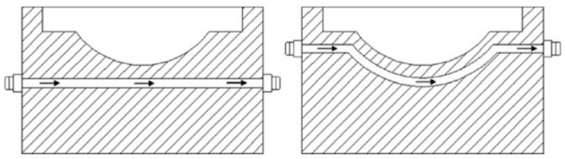
\includegraphics{media/cooling_channels.png}
            \end{adjustbox}
            \caption{\label{fig:cooling_channels}Canales de enfriamiento convencionales y conformes.}
            Fuente: \textcite{Shinde2017}
            \end{figure}
        
            \item \textbf{\textit{Tubo de Calor}:} Los tubos de calor (\cite{richard1944gaugler}), son un eficaz dispositivo de intercambio de calor, han captado la atención de la comunidad de transferencia de calor debido a su sencilla estructura, alta confiabilidad y eficaz capacidad de transferencia de calor, los tubos de calor se han convertido en una elección común en la gestión térmica de dispositivos electrónicos de alta potencia.
        
        \end{enumerate}
        
\end{enumerate}
\end{enumerate}

\needspace{4cm}
\subsubsection{Comparación de Productos Relacionados}
Se revisó una serie de cámaras inteligentes con características interesantes para el desarrollo del producto planteado, se puede apreciar a las mismas en las Figuras \ref{fig:EZVIC_C2C} a \ref{fig:ReolinkArgusP}.

\begin{enumerate}[label=\alph*)]
    \needspace{3cm}
    \item EZVIZ C2C
    
    \begin{figure}[H]
    \centering
    \begin{adjustbox}{width=\linewidth/2}
      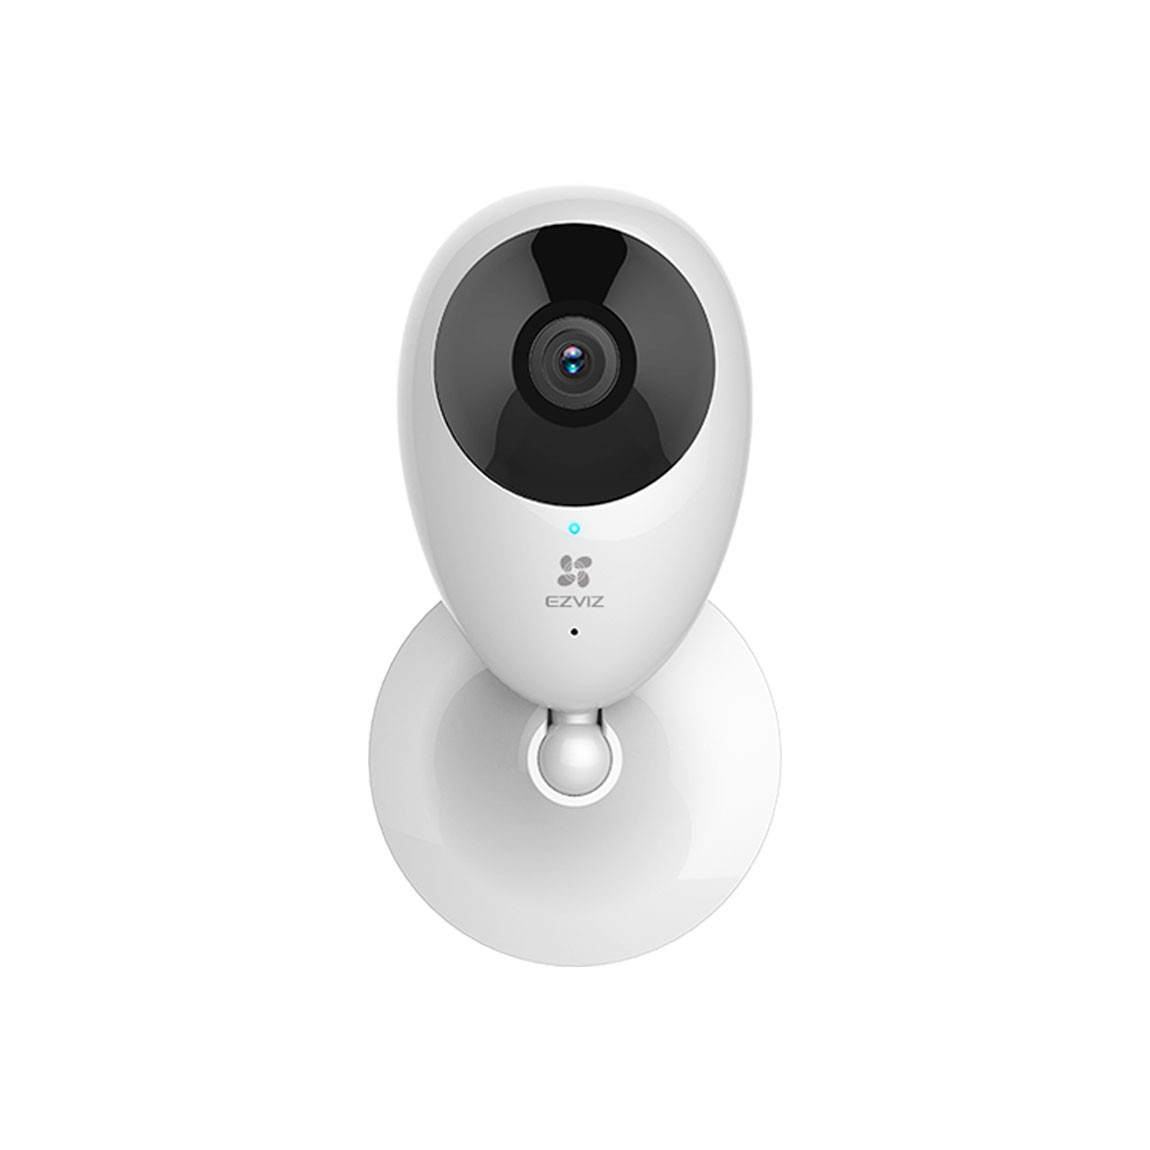
\includegraphics{media/ezvic_c2c.jpeg}
    \end{adjustbox}
    \caption{\label{fig:EZVIC_C2C}Cámara inteligente EZVIC C2C.}
    \end{figure}
    
    La cámara presente en la Figura \ref{fig:EZVIC_C2C}, está diseñada para una instalación rápida y sencilla gracias a su base magnética(\cite{EZVIZ}). Desventaja: No tiene movimiento automático, depende del usuario o transeúnte.

    \needspace{3cm}
    \item Imou

    \begin{figure}[H]
    \centering
    \begin{adjustbox}{width=\linewidth/4}
          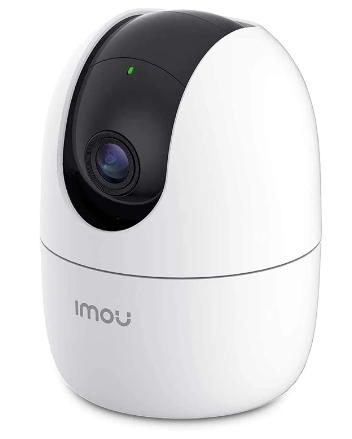
\includegraphics{media/Imou.png}
    \end{adjustbox}
    \caption{\label{fig:Imou}Cámara inteligente Imou.}
    \end{figure}

    Una de las características más destacables de este producto es que su cámara con sensor de movimiento es capaz de detectar cualquier intrusión en segundos, realizar un seguimiento automático de la actividad y grabar vídeos en tiempo real. 

    \needspace{3cm}
    \item Xiaomi Domo

    \begin{figure}[H]
    \centering
    \begin{adjustbox}{width=\linewidth/4}
      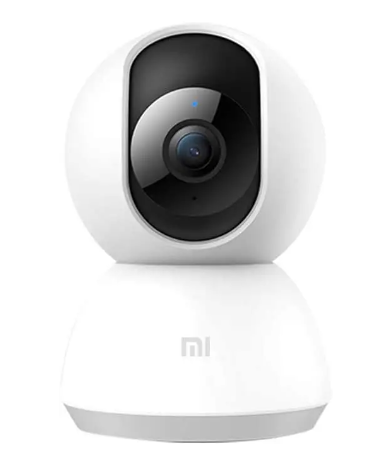
\includegraphics{media/XiaomiDomo.png}
    \end{adjustbox}
    \caption{Cámara inteligente Xiaomi Domo.}
    \label{fig:XiamiDomo}
    \end{figure}

    La cámara cuenta con un rango de rotación horizontal de 360º y vertical de 96º. 
    Tiene motores duales silenciosos, los lentes de la cámara rotan en completo silencio para pasar inadvertida hasta en las horas de sueño profundo. De hecho, esta cámara puede instalarse de lado, en posición invertida o sencillamente sobre un estante, puesto que su base es sólida e incluye tornillos para un ajuste firme.

    \needspace{3cm}
    \item Reolink Argus P

    \begin{figure}[H]
    \centering
    \begin{adjustbox}{width=\linewidth/2}
      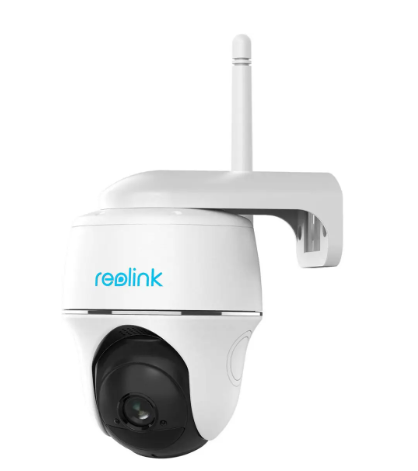
\includegraphics{media/reolink.png}
    \end{adjustbox}
    \caption{\label{fig:ReolinkArgusP}Cámara inteligente Reolink Argus P.}
    \end{figure}

    Ofrece un amplio ángulo de visión puesto que su lente gira 355º en sentido horizontal y 140º verticalmente.
    
\end{enumerate}

\needspace{5cm}
\subsection{Búsqueda Interna}
\begin{enumerate}[label=\alph*)]

\item \textbf {Administración de energía:} Diseño de un sistema de administración de energía eficiente que permita un funcionamiento continuo en interiores y la recarga de baterías cuando sea necesario.
    \begin{itemize}
    \item Uso de paneles solares para cargar las baterías y proporcionar energía sostenible.
    \item Incorporación de una función de ahorro de energía que apague automáticamente la detección cuando no se detecta actividad de fumado durante un período prolongado.
    \item Posibilidad de alimentación a través de la red eléctrica para su uso en lugares donde haya acceso a tomas de corriente.
    \end{itemize}

\item \textbf{Sistema de movimiento:} Desarrollo de un sistema de orientación de cámara con movimientos suaves y discretos para evitar molestar a las personas en interiores.
    \begin{itemize}
    \item Uso de sensores de proximidad para garantizar que la cámara no colisione con objetos o paredes mientras se ajusta para obtener una vista óptima.
    \item Implementación de un modo de seguimiento silencioso que minimice cualquier ruido mecánico al seguir a una persona fumando.
    \item Diseño de un mecanismo de montaje versátil que permita la instalación en techos, paredes o esquinas de interiores.
    \end{itemize}

\item \textbf{Gestión Térmica:} Diseño de conductos de aire ajustables que permitan direccionar el flujo de aire hacia las áreas donde se detecta actividad de fumado en interiores.
    \begin{itemize}
    \item Integración de ventiladores de baja sonoridad para mantener un ambiente tranquilo y cómodo en lugares cerrados.
    \item Uso de sensores de temperatura y humedad para ajustar la velocidad y dirección del flujo de aire de acuerdo con las condiciones ambientales.
    \item Desarrollo de una carcasa compacta y estética que se integre de manera discreta en entornos interiores.
    \item Diseño de generadores de vórtices para maximizar la entropía en los conductos de ventilación, sabiendo que la entropía maximiza la disipación del calor.
    \end{itemize}
\end{enumerate}

    \needspace{3cm}
    \subsection{Exploración Sistemática}
    
    \subsubsection{Árbol de Clasificación}

    \begin{figure}[H]
        \centering
        \resizebox{0.5\linewidth}{!}{
            \begin{tikzpicture}[mindmap, grow cyclic, every node/.style=concept, concept color=olive!40,
                level 1/.append style={level distance=6cm,sibling angle=100},
                level 2/.append style={level distance=3cm,sibling angle=39},
            ]
            % Root concept
            \node[concept] {Distribucion de Energia}
            child [concept color=red!40] {
                node[concept] {Gestión de Cables}
                child { node[concept] {Arandelas} }
                child { node[concept] {Clips} }
                child { node[concept] {Correas} }
                child { node[concept] {Monturas para Correas} }
                child { node[concept] {Envolturas y Fundas} }
                child { node[concept] {Glandes} }
                child { node[concept] {Tubos termoretráctiles} }
                child { node[concept] {Correas de torsión} }
                child { node[concept] {Abrazaderas} }
            }
            child [concept color=teal!40, level distance=4.2cm] {
                node[concept] {Selección de Baterías}
                child { node[concept] {Alcalinas} }
                child { node[concept] {De botón} }
                child { node[concept] {Plomo-Acido} }
                child { node[concept] {NiCd} }
                child { node[concept] {NiMH} }
                child { node[concept] {Li-Ion} }
            };
        \end{tikzpicture}
        }
        \caption{Árbol de clasificación para los fragmentos de concepto del sistema de conversión de energía.}
        \label{fig:arbolEnergia}
    \end{figure}


    El diagrama de la Figura \ref{fig:arbolEnergia} muestra una jerarquía de conceptos relacionados con la "Distribución de Energía". Hay dos categorías principales: "Gestión de Cables" en azul y "Selección de Baterías" en verde. "Gestión de Cables" se desglosa en subconceptos como "Protección de Cables" y "Orientación de Cables", mientras que "Selección de Baterías" incluye "Tipo de Batería" y "Capacidad y Duración". Este gráfico ayuda a comprender los elementos clave de un sistema de distribución de energía.
    
    \begin{figure}[H]
    \centering
    \resizebox{0.6\linewidth}{!}{
    \begin{tikzpicture}[mindmap, grow cyclic, every node/.style=concept, concept color=red!40,
        level 1/.append style={level distance=5cm,sibling angle=90},
        level 2/.append style={level distance=4cm,sibling angle=45},
        ]
        % Root concept
        \node[concept] {Sistemas de Movimiento}
        child [concept color=orange!40, level distance=4.5cm] {
            node[concept] {Selección de Motor}
            child { node[concept] {Motor DC} }
            child { node[concept] {Motor Brushless} }
            child { node[concept] {Motor a Paso} }
            child { node[concept] {Servomotor} }
        }
        child [concept color=magenta!40, level distance=5.4cm] {
            node[concept] {Generadores de Movimiento Panorámico y de Inclinación (PTMG)}
            child { node[concept] {Tren de Engranes Cónicos} }
            child { node[concept] {Juntas Homocinéticas} }
            child { node[concept] {Mecanismo de Cinco Barras} }
            child { node[concept] {Enlace Esférico} }
            child { node[concept] {Tren de Engranes Diferencial} }
            child { node[concept] {Mecanismo de Hervé} }
        };
    \end{tikzpicture}
    }
    \caption{\label{fig:arbolClasificacionMovimiento} Árbol de clasificación para los fragmentos de concepto del sistema de transformación de movimiento.}
    \label{fig:arbolMovimiento}
    \end{figure}

    El gráfico de la Figura \ref{fig:arbolMovimiento} muestra una estructura jerárquica de conceptos relacionados con sistemas de movimiento. En la raíz, está "Sistemas de Movimiento", que se divide en dos categorías principales: "Selección de Motor" y "Generadores de Movimiento Panorámico y de Inclinación (PTMG)". Cada categoría tiene subconceptos específicos. Por ejemplo, en "Selección de Motor", se incluyen "Motor DC", "Motor Brushless", "Motor a Paso" y "Servomotor". Mientras que en "Generadores de Movimiento Panorámico y de Inclinación (PTMG)", se presentan conceptos como "Tren de Engranes Cónicos" y otros.

    \begin{figure}[H]
    \centering
    \resizebox{0.6\linewidth}{!}{
    \begin{tikzpicture}[mindmap, grow cyclic, every node/.style=concept, concept color=violet!40,
        level 1/.append style={level distance=5cm,sibling angle=65}, % Growing upward
        level 2/.append style={level distance=4.2cm,sibling angle=50},
    ]
    % Root concept
    \node[concept] {Gestión Térmica}
        child [concept color=blue!40] { 
            node[concept] {Ventilación de Aire de adelante hacia atrás}
            child { node[concept] {Ventiladores en la Parte Trasera} }
            child { node[concept] {Montaje Horizontal de Placas Electrónicas} }
            child { node[concept] {Montaje Vertical de Placas Electrónicas} }
            child { node[concept] {Ventiladores Directamente Encima de las Placas Electrónicas:} }
        }
        child [concept color=cyan!40] { 
            node[concept] {Indirecta} 
            child { node[concept] {Canales de Refrigeración} }
            child { node[concept] {Tubo de calor} }
        };
    \end{tikzpicture}
    }
    \caption{Árbol de clasificación para los fragmentos de concepto del sistema de gestión térmica.}
    \label{fig:arbolAire}
    \end{figure}

    El diagrama de la figura \ref{fig:arbolAire} representa una jerarquía de conceptos relacionados con el "Direccionamiento de Aire". En la raíz del árbol se encuentra este concepto principal, que se divide en cuatro subconceptos: "Optimización de Diseño", "Canal de Refrigeración", "Geometría Compleja" y "Enfriamiento Uniforme". Este gráfico proporciona una estructura visual para comprender los aspectos clave del sistema de gestión térmica.
    
    \needspace{2.5cm}
    \subsubsection{Tablas de Combinación}

    \begin{table}[H]
    \centering
    \begin{tabularx}{\textwidth}{|X|X|X|X|X|}
    \hline
    \textbf{Convertir Energía Eléctrica en Energía Mecánica} & \textbf{Aplicar Energía Mecánica al Mecanismo} & \textbf{Selección de Baterías} & \textbf{Gestión de Cables} & \textbf{Gestion Termica} \\
    \hline
    Motor paso a paso & Mecanismo de Hervé & \cellcolor{green}Li-Ion  & Arandelas & Tubo de calor\\
    \hline
    \cellcolor{green}Motor Brushless & \cellcolor{green}Tren de engranes diferencial & NiMH & Clips & Canales de Refrigeracion \\
    \hline
    Motor DC & Enlace Esférico & NiCd & Correas & \cellcolor{green}Ventiladores encima de las placas electronicas\\
    \hline
    Servomotor & Mecanismo de cinco barras & Plomo-Acido & Monturas para correas & Montaje vertical de las placas electronicas\\
    \hline
     & Juntas Homocinéticas & De boton & Encolturas y fundas & Montaje Horizontal de las placas electronicas\\
    \hline
     & Tren de Engranes Cónicos & Alcalinas & Glandes & Ventiladores en la parte trasera\\
    \hline
     & & & \cellcolor{green}Abrazadera para cables & \\
    \hline
     & & & Tubos termoretractiles & \\
    \hline
     & & & Correas de torsion & \\
    \hline
    \end{tabularx}
    \caption{Tabla de Combinación 1}
    \label{tab:combinacion_1}
    \end{table}

    En el Cuadro \ref{tab:combinacion_1}, se presenta una solución elegante que combina un motor brushless con el sofisticado mecanismo de un tren de engranes diferencial. Esta configuración es alimentada por baterías Li-Ion, y la organización ordenada de los cables mediante abrazaderas asegura un aspecto limpio y profesional. Además, se han incorporado ventiladores estratégicamente ubicados encima de las placas electrónicas para disipar el calor.
    
    \begin{table}[H]
    \centering
    \begin{tabularx}{\textwidth}{|X|X|X|X|X|}
    \hline
    \textbf{Convertir Energía Eléctrica en Energía Mecánica} & \textbf{Aplicar Energía Mecánica al Mecanismo} & \textbf{Selección de Baterías} & \textbf{Gestión de Cables} & \textbf{Gestion Termica} \\
    \hline
    Motor paso a paso & Mecanismo de Hervé & \cellcolor{green}Li-Ion  & Arandelas & Tubo de calor\\
    \hline
    Motor Brushless & Tren de engranes diferencial & NiMH & Clips & Canales de Refrigeracion \\
    \hline
    Motor DC & Enlace Esférico & NiCd & Correas & \cellcolor{green}Ventiladores encima de las placas electronicas\\
    \hline
    \cellcolor{green}Servomotor & Mecanismo de cinco barras & Plomo-Acido & Monturas para correas & Montaje vertical de las placas electronicas\\
    \hline
     & Juntas Homocinéticas & De boton & Encolturas y fundas & Montaje Horizontal de las placas electronicas\\
    \hline
     & \cellcolor{green}Tren de Engranes Cónicos & Alcalinas & Glandes & Ventiladores en la parte trasera\\
    \hline
     & & & \cellcolor{green}Abrazadera para cables & \\
    \hline
     & & & Tubos termoretractiles & \\
    \hline
     & & & Correas de torsion & \\
    \hline
    \end{tabularx}
    \caption{Tabla de Combinación 2}
    \label{tab:combinacion_2}
    \end{table}

    El Cuadro \ref{tab:combinacion_2} muestra una solución que combina un servomotor con un tren de engranes cónicos. Se alimenta con baterías Li-Ion y utiliza abrazaderas para mantener los cables organizados. Además, se han colocado ventiladores sobre las placas electrónicas para reducir la temperatura.

    \begin{table}[H]
    \centering
    \begin{tabularx}{\textwidth}{|X|X|X|X|X|}
    \hline
    \textbf{Convertir Energía Eléctrica en Energía Mecánica} & \textbf{Aplicar Energía Mecánica al Mecanismo} & \textbf{Selección de Baterías} & \textbf{Gestión de Cables} & \textbf{Gestion Termica} \\
    \hline
    Motor paso a paso & Mecanismo de Hervé & \cellcolor{green}Li-Ion  & Arandelas & Tubo de calor\\
    \hline
    Motor Brushless & \cellcolor{green}Tren de engranes diferencial & NiMH & Clips & Canales de Refrigeracion \\
    \hline
    \cellcolor{green}Motor DC & Enlace Esférico & NiCd & Correas & \cellcolor{green}Ventiladores encima de las placas electronicas\\
    \hline
    Servomotor & Mecanismo de cinco barras & Plomo-Acido & Monturas para correas & Montaje vertical de las placas electronicas\\
    \hline
     & Juntas Homocinéticas & De boton & Encolturas y fundas & Montaje Horizontal de las placas electronicas\\
    \hline
     & Tren de Engranes Cónicos & Alcalinas & Glandes & Ventiladores en la parte trasera\\
    \hline
     & & & \cellcolor{green}Abrazadera para cables & \\
    \hline
     & & & Tubos termoretractiles & \\
    \hline
     & & & Correas de torsion & \\
    \hline
    \end{tabularx}
    \caption{Tabla de Combinación 3}
    \label{tab:combinacion_3}
    \end{table}    

    El Cuadro \ref{tab:combinacion_3} muestra una solución que combina un motor de corriente continua con un tren de engranes diferencial. Se alimenta con baterías Li-Ion y utiliza abrazaderas para mantener los cables organizados. Además, se han colocado ventiladores sobre las placas electrónicas para disipar el calor.

    \begin{table}[H]
    \centering
    \begin{tabularx}{\textwidth}{|X|X|X|X|X|}
    \hline
    \textbf{Convertir Energía Eléctrica en Energía Mecánica} & \textbf{Aplicar Energía Mecánica al Mecanismo} & \textbf{Selección de Baterías} & \textbf{Gestión de Cables} & \textbf{Gestion Termica} \\
    \hline
    \cellcolor{green}Motor paso a paso & Mecanismo de Hervé & \cellcolor{green}Li-Ion  & Arandelas & Tubo de calor\\
    \hline
    Motor Brushless & Tren de engranes diferencial & NiMH & Clips & \cellcolor{green}Canales de Refrigeracion \\
    \hline
    Motor DC & Enlace Esférico & NiCd & \cellcolor{green}Correas & Ventiladores encima de las placas electronicas\\
    \hline
    Servomotor & Mecanismo de cinco barras & Plomo-Acido & Monturas para correas & Montaje vertical de las placas electronicas\\
    \hline
     & Juntas Homocinéticas & De boton & Encolturas y fundas & Montaje Horizontal de las placas electronicas\\
    \hline
     & \cellcolor{green}Tren de Engranes Cónicos & Alcalinas & Glandes & Ventiladores en la parte trasera\\
    \hline
     & & & Abrazadera para cables & \\
    \hline
     & & & Tubos termoretractiles & \\
    \hline
     & & & Correas de torsion & \\
    \hline
    \end{tabularx}
    \caption{Tabla de Combinación 4}
    \label{tab:combinacion_4}
    \end{table} 

    El Cuadro \ref{tab:combinacion_4} muestra una solución que combina un motor paso a paso con un tren de engranes conicos. Se alimenta con baterías Li-Ion y utiliza correas para mantener los cables organizados. Además, se incorpora canales de refrigeracion para difundir el calor.

    \begin{table}[H]
    \centering
    \begin{tabularx}{\textwidth}{|X|X|X|X|X|}
    \hline
    \textbf{Convertir Energía Eléctrica en Energía Mecánica} & \textbf{Aplicar Energía Mecánica al Mecanismo} & \textbf{Selección de Baterías} & \textbf{Gestión de Cables} & \textbf{Gestion Termica} \\
    \hline
    Motor paso a paso & Mecanismo de Hervé & Li-Ion  & Arandelas & Tubo de calor\\
    \hline
    Motor Brushless & Tren de engranes diferencial & NiMH & Clips & Canales de Refrigeracion \\
    \hline
    Motor DC & Enlace Esférico & NiCd & Correas & Ventiladores encima de las placas electronicas\\
    \hline
    \cellcolor{green}Servomotor & \cellcolor{green}Mecanismo de cinco barras & \cellcolor{green}Plomo-Acido & Monturas para correas & Montaje vertical de las placas electronicas\\
    \hline
     & Juntas Homocinéticas & De boton & Encolturas y fundas & Montaje Horizontal de las placas electronicas\\
    \hline
     & Tren de Engranes Cónicos & Alcalinas & Glandes & \cellcolor{green}Ventiladores en la parte trasera\\
    \hline
     & & & Abrazadera para cables & \\
    \hline
     & & & \cellcolor{green}Tubos termoretractiles & \\
    \hline
     & & & Correas de torsion & \\
    \hline
    \end{tabularx}
    \caption{Tabla de Combinación 5}
    \label{tab:combinacion_5}
    \end{table} 

    El Cuadro \ref{tab:combinacion_5} muestra una solución que combina un servomotor con un mecanimso de cinco barras. Se alimenta con baterías Plomo-Acido y utiliza tubos termoretractiles para mantener los cables organizados y seguros. Además, se incorpora ventiladores en la parte trasera para evacuar el calor.

    \begin{table}[H]
    \centering
    \begin{tabularx}{\textwidth}{|X|X|X|X|X|}
    \hline
    \textbf{Convertir Energía Eléctrica en Energía Mecánica} & \textbf{Aplicar Energía Mecánica al Mecanismo} & \textbf{Selección de Baterías} & \textbf{Gestión de Cables} & \textbf{Gestion Termica} \\
    \hline
    Motor paso a paso & \cellcolor{green}Mecanismo de Hervé & \cellcolor{green}Li-Ion  & Arandelas & Tubo de calor\\
    \hline
    Motor Brushless & Tren de engranes diferencial & NiMH & Clips & Canales de Refrigeracion \\
    \hline
    \cellcolor{green}Motor DC & Enlace Esférico & NiCd & \cellcolor{green}Correas & Ventiladores encima de las placas electronicas\\
    \hline
    Servomotor & Mecanismo de cinco barras & Plomo-Acido & Monturas para correas & Montaje vertical de las placas electronicas\\
    \hline
     & Juntas Homocinéticas & De boton & Encolturas y fundas & Montaje Horizontal de las placas electronicas\\
    \hline
     & Tren de Engranes Cónicos & Alcalinas & Glandes & \cellcolor{green}Ventiladores en la parte trasera\\
    \hline
     & & & Abrazadera para cables & \\
    \hline
     & & & Tubos termoretractiles & \\
    \hline
     & & & Correas de torsion & \\
    \hline
    \end{tabularx}
    \caption{Tabla de Combinación 6}
    \label{tab:combinacion_6}
    \end{table} 

    El Cuadro \ref{tab:combinacion_6} muestra una solución que combina un motor de corriente continua con un mecanimso de Hervé. Se alimenta con baterías de Li-Ion y utiliza tubos correas para cables, manteniendo en orden el cableado interno. Además, se incorpora ventiladores en la parte trasera para evacuar el calor.

\needspace{3cm}
\subsection{Análisis de Soluciones}
\subsubsection{Explorar el espacio de solucion}
    Dentro del marco de este proyecto, se llevó a cabo una exhaustiva exploración de diversas soluciones destinadas a abordar las problemáticas planteadas. Cada una de estas opciones se describe con detalle en este informe. A medida que avanzaba la investigación, se recibía retroalimentación que aportaba nuevas ideas para investigar y ayudaba a descartar las soluciones menos eficientes. Este enfoque de refinamiento constante ha contribuido a la evolución y optimización de las estrategias, asegurando que cada elección esté respaldada por un análisis riguroso y contribuya al éxito global del proyecto.
\subsubsection{Revisar alternativa}
    Dentro del ámbito de este proyecto, se llevó a cabo una meticulosa revisión de alternativas con el objetivo de abordar las problemáticas planteadas. Este informe presenta un análisis exhaustivo de cada una de las opciones consideradas. En el transcurso de la investigación, surgieron preguntas fundamentales, como si existían diagramas funcionales alternativos o si era posible una descomposición del problema desde enfoques diferentes. Esta perspicaz línea de indagación permitió explorar nuevas vías que podrían conducir a soluciones potencialmente más eficaces. El proceso de revisión constante, en combinación con un análisis crítico y creativo, ha sido esencial para refinar y optimizar nuestras estrategias, garantizando que cada elección se base en una evaluación sólida y contribuya al éxito global del proyecto.
\subsubsection{Considerar fuentes externas}
    Dentro del contexto de este proyecto, se ha llevado a cabo una exhaustiva evaluación de fuentes externas pertinentes, incluyendo literatura técnica e investigaciones previas. Esta revisión meticulosa ha permitido enriquecer las soluciones propuestas y tomar decisiones más sólidas y fundamentadas. El proceso de consideración de fuentes externas ha sido esencial para optimizar las estrategias, asegurando que cada elección esté respaldada por una base de conocimiento sólida y contribuya al éxito general del proyecto.
\subsubsection{Integrar ideas}
    Dentro del marco de este proyecto, se ha puesto un especial énfasis en la integración de ideas y contribuciones de todo el equipo. Cada idea, aportación y perspectiva ha sido considerada de manera meticulosa y se ha trabajado de forma efectiva para su incorporación adecuada en el proceso. La colaboración constante y la comunicación efectiva entre los miembros del equipo han sido fundamentales en este paso, asegurando que todas las voces sean escuchadas y que las ideas se integren de manera armoniosa y productiva.